\documentclass[aspectratio=169]{beamer}
\usepackage{tikz}
\usetikzlibrary{arrows.meta}
\setbeamertemplate{navigation symbols}{}

\title{Equity Allocation Under a Terminal Wealth Floor}
\author{Yuru Lin, Ryan Tomich, Moritz Wassermann}
\date{}

\begin{document}

\begin{frame}[plain]
  \titlepage
\end{frame}

\begin{frame}{Objective and Constraints}
    Start with \$100M in cash. The horizon \(T\) is set at launch (1--2 years).

    \medskip
    \begin{itemize}
        \setlength{\itemsep}{0.8em}
        \item \textbf{Objective.} Maximize certainty-equivalent terminal wealth
            (\(\gamma=2\)). For each launch condition \(s\), report
            \(\mathrm{CE}_s=1/\mathbb{E}[1/W_T\mid s]\).
        \item \textbf{Floor.} Require \(\Pr(W_T<\$95\mathrm{M}\mid s)\le 2\%\)
            in each launch condition.
        \item \textbf{Trading.} Rebalance daily between diversified equity and
            interest-bearing cash. Equity weight \(0\)--\(100\%\). Negligible costs.
        \item \textbf{Launch condition \(s\).} Classify using data through the prior close.
            \begin{itemize}
                \item \textbf{Crisis:} equity index at least 20\% below its trailing 12-month high.
                \item \textbf{High volatility:} outside crisis, 63-session equity return volatility
                    above its historical median.
                \item \textbf{Normal volatility:} outside crisis, volatility at or below that median.
            \end{itemize}
    \end{itemize}
\end{frame}

\begin{frame}{Full DP}
    % Full DP method diagram, drawn in the presentation's Beamer colors.
\begingroup
\usebeamercolor{structure}
\colorlet{dpblue}{structure.fg}
\centering
\begin{tikzpicture}[
    x=1cm, y=1cm, font=\scriptsize,
    heading/.style={text=dpblue, font=\small\bfseries},
    label/.style={font=\scriptsize\bfseries},
    box/.style={draw=dpblue!45, fill=dpblue!4, rounded corners=2pt,
                align=center, inner xsep=4pt, inner ysep=3pt},
    link/.style={-{Stealth[length=1.4mm]}, draw=black!65, thin},
    note/.style={anchor=north west, align=left, inner sep=0pt}
]
% A two-session decision in the baseline model.
\node[heading, anchor=west] at (0,6.32) {Regular DP};
\node[anchor=east] at (13.8,6.32)
    {$\displaystyle J_d(s)=\max_{a\in A(s)}\sum_{s'}p(s'\mid s,a)\,J_{d-1}(s')$};

\node[label] at (1.20,5.66) {Current state};
\node[label] at (4.29,5.66) {Equity decision};
\node[label] at (8.65,5.66) {Next state};
\node[label] at (12.05,5.66) {Continuation value};
\node[box] (state) at (1.20,4.47)
    {\$96M wealth\\Ordinary volatility\\2 sessions left};
\node[box] (action) at (4.29,4.47)
    {$a\in\{0,.25,.5,.75,1\}$\\Example: $a=.75$};
\draw[link] (state) -- (action);

\coordinate (fork) at (5.85,4.47);
\draw[black!65] (action.east) -- (fork);
\foreach \i/\y/\wealth/\regime/\prob in {
    1/5.19/95.34/ordinary/49.5, 2/4.71/95.34/high/0.5,
    3/4.23/96.70/ordinary/49.5, 4/3.75/96.70/high/0.5}{
    \node[box, minimum width=2.52cm, inner ysep=1.8pt] (s\i) at (8.65,\y)
        {\$\wealth M, \regime};
    \draw[link] (fork) -- (6.34,\y) -- (s\i.west)
        node[midway, fill=white, inner sep=1pt] {\prob\%};
    \node (v\i) at (12.05,\y) {$J_{d-1}(s'_{\i})$};
    \draw[link] (s\i.east) -- (v\i.west);
    \draw[dpblue!65] (v\i.east) -- (13.22,\y);
}
\draw[dpblue!65] (13.22,5.19) -- (13.22,3.75);
\draw[link, draw=dpblue!65, rounded corners=2pt]
    (13.22,3.75) -- (13.22,3.21) -- (4.29,3.21) -- (action.south);
\node[fill=white, text=dpblue, inner xsep=4pt] at (8.65,3.21)
    {Weight by probability};

% The three changes from regular DP to Full DP.
\draw[black!22] (0,2.90) -- (13.8,2.90);
\foreach \x/\title in {0/Equity cap,4.75/Downside shocks,9.38/Policy selection}
    \node[heading, anchor=west, inner xsep=0pt] at (\x,2.57) {\title};
\node[note, text width=4.38cm] at (0,2.17)
    {Limit equity using the cushion above the \$95M floor.
     With $C=(W-F)_+$ and $K=\$5\mathrm{M}$,\\[4pt]
     $E_{\max}=\min\{W,\,m\min(C,K)$\\
     $\hphantom{E_{\max}=\min\{W,\,}{}+1.5m(C-K)_+\}$.\\[5pt]
     At \$96M with $m=8$, equity is capped at \textbf{\$8M}.};

\node[note, text width=4.12cm] at (4.75,2.17)
    {Add a rare loss to each regime. Ordinary-regime outcomes:};
\coordinate (shock) at (5.02,0.90);
\fill[dpblue] (shock) circle (1.8pt);
\foreach \y/\outcome in {1.38/{Up \enspace(49.95\%)},
                         0.90/{Down \enspace(49.95\%)},
                         0.42/{Crash \enspace(0.10\%, $-10\%$)}}{
    \node[box, anchor=west, inner ysep=1.8pt] (outcome) at (5.68,\y) {\outcome};
    \draw[link] (shock) -- (outcome.west);
}
\node[note, text width=4.35cm] at (9.38,2.17)
    {At launch, compare four penalty policies and cash. Maximize expected terminal wealth among those with breach risk below 2\%.\\[5pt]
     $\displaystyle \pi^*\in\arg\max_{\pi\in\Pi}\mathbb E_\pi[W_T\mid s_0]$\\[3pt]
     $\text{s.t.}\quad\Pr_\pi(W_T<F\mid s_0)<2\%$.};
\end{tikzpicture}\par
\endgroup

\end{frame}

\begin{frame}{Volatility-Capped Smooth Cushion}
    Full DP can jump at a volatility cutoff. A smooth rule adjusts equity gradually.

    \medskip
    \begin{enumerate}
        \item \textbf{Fund the floor.} With \(n\) days left at daily cash rate \(r_f\),
        \[
            \text{Reserve } R=\frac{\$95\text{M}}{(1+r_f)^n},
            \qquad \text{cushion } C=\max(W-R,0).
        \]

        \item \textbf{Size equity.} Each extra cushion dollar adds \$1 to \$4 of base
        equity as \(C\) grows. Scale down for higher volatility and divide by wealth
        \(W\) to get target weight \(q\).

        \medskip
        \item \textbf{Cap smoothly.} At annualized volatility \(\sigma\),
        \[
            \text{Ceiling } h=\frac{1}{1+(\sigma/0.30)^4},
            \qquad \text{equity weight } w=\frac{q}{(1+(q/h)^4)^{1/4}}.
        \]
        For \(q\ll h\), \(w\approx q\). For \(q\gg h\), \(w\approx h\).
        At 30\% volatility, \(h=50\%\).
    \end{enumerate}
\end{frame}

\begin{frame}{Equity Allocation: Smooth Cushion Adjusts Exposure Gradually}
    \centering
    % Align headings with the plot panels, leaving room for the axes and colorbar.
    \makebox[\linewidth][l]{\large\bfseries\usebeamercolor[fg]{structure}%
        \hspace*{0.035\linewidth}%
        \makebox[0.288\linewidth]{Regular DP}%
        \makebox[0.288\linewidth]{Full DP}%
        \makebox[0.288\linewidth]{Smooth}}\par
    \smallskip
    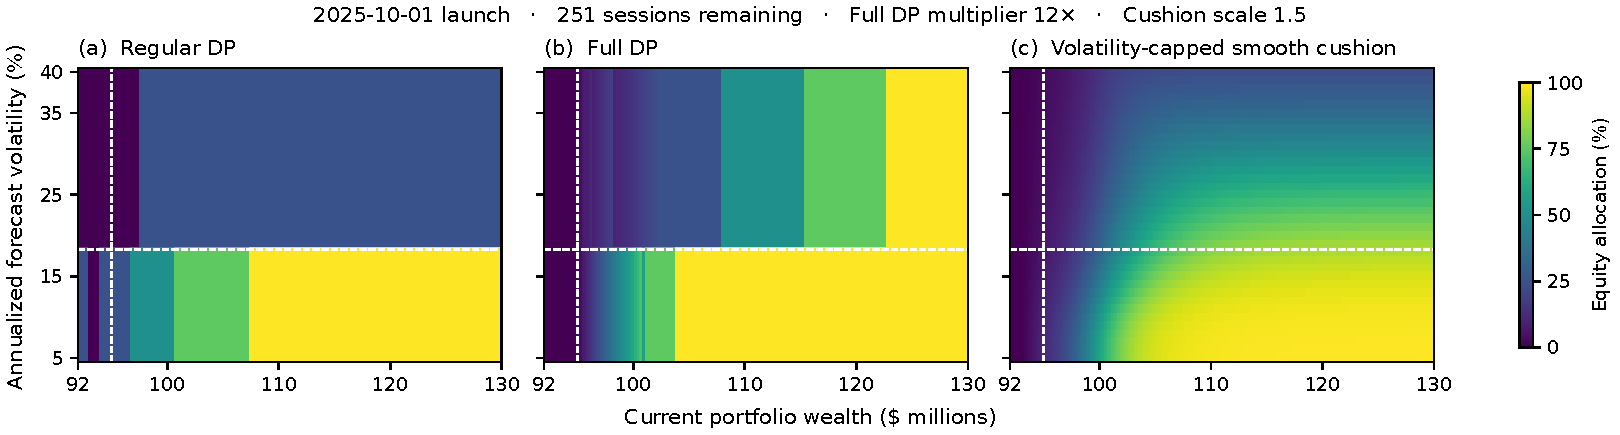
\includegraphics[width=\linewidth]{figures/slide-heatmaps.pdf}

    \smallskip
    {\footnotesize Dashed lines mark the \$95M floor and the launch volatility cutoff.\par}
\end{frame}

\begin{frame}{Certainty-Equivalent Wealth: Full DP Leads Overall}
    \begin{columns}[c,onlytextwidth]
        \begin{column}{0.58\textwidth}
            \centering
            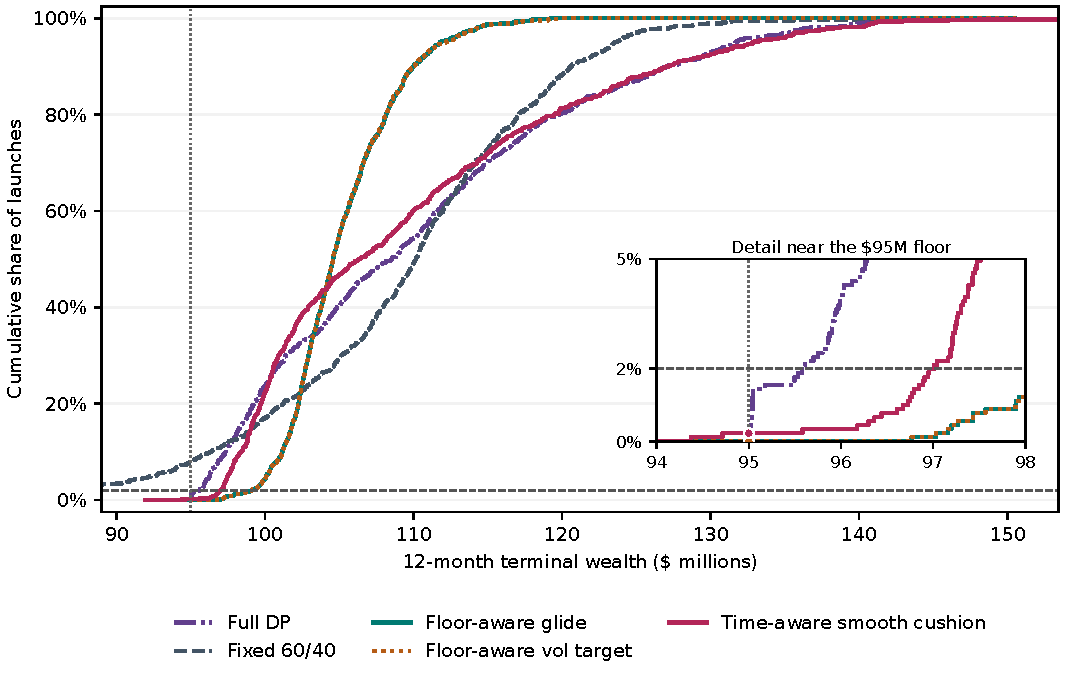
\includegraphics[width=\linewidth]{figures/alternatives-cdf.pdf}
            \par\smallskip
            {\small\(\displaystyle
                \mathrm{CE}=\left(\frac{1}{n}\sum_{i=1}^{n}\frac{1}{W_{T,i}}\right)^{-1}
            \)\par}
        \end{column}
        \begin{column}{0.40\textwidth}
            \centering\footnotesize
            \setlength{\tabcolsep}{3pt}
            \renewcommand{\arraystretch}{0.90}
            \begin{tabular}{@{}lrr@{}}
\hline
Strategy & CE (\$M) & Breach rate \\
\hline
\multicolumn{3}{@{}l}{\itshape All launches ($n=910$)} \\
Regular DP & 109.02 & 2.97\% \\
Full DP & \textbf{109.07} & 0.11\% \\
Vol.-capped cushion & 108.37 & \textbf{0.00\%} \\
\hline
\multicolumn{3}{@{}l}{\itshape Lower volatility ($n=440$)} \\
Regular DP & \textbf{108.98} & 2.73\% \\
Full DP & 108.90 & 0.23\% \\
Vol.-capped cushion & 108.31 & \textbf{0.00\%} \\
\hline
\multicolumn{3}{@{}l}{\itshape Higher volatility ($n=416$)} \\
Regular DP & 108.72 & 3.12\% \\
Full DP & \textbf{108.90} & \textbf{0.00\%} \\
Vol.-capped cushion & 108.11 & \textbf{0.00\%} \\
\hline
\multicolumn{3}{@{}l}{\itshape Crisis ($n=54$)} \\
Regular DP & 111.72 & 3.70\% \\
Full DP & \textbf{111.92} & \textbf{0.00\%} \\
Vol.-capped cushion & 110.92 & \textbf{0.00\%} \\
\hline
\end{tabular}

        \end{column}
    \end{columns}
    \medskip
    {\footnotesize Monthly launches from January 1950 through October 2025 each ran for \(T=12\) months.\\
    \(W_{T,i}\) is terminal wealth for launch \(i\). A breach occurs if \(W_{T,i}<\$95\text{M}\).\par}
\end{frame}

\end{document}
